\section{Overview of the Microcode Engine}

One of the first decisions
- hardware performance, software flexibility \cite{}
- hardware fast\\
- software flexible\\
- microcode engine: basic instructions to gain some amount of flexibility\\

\subsection{Instruction Set}

The MCE implements a set of microcode instructions, which is displayed in table~\ref{tab:mce_isa}.
The opcode identifying an instruction is 8~bit wide.
It consists of two 4~bit elements called \emph{major opcode} and \emph{minor opcode}.
Thereby, the major opcode forms a group of similar instructions and the minor opcode identifies a specific instruction inside of such a group.\\
Furthermore, an instruction can access up to three registers of the scratchpad.
4~bit addresses are used for this purpose.
The \emph{RD} field specifies the address of the destination register, where the result of the operation is stored.
The addresses of the source operands are determined by \emph{RS1} and \emph{RS2}.
Values can also directly be included in instructions.
The \emph{immediate} field is used for this.\\
Additionally to the result of the operation itself, an instruction can produce a condition code, which is written into the condition code register (CCR).
The address of the register is specified by the 2~bit field \emph{crs}.
The condition code can then be used in other instructions.
Therefor, the 4~bit wide \emph{ccmux} field is used.
It addresses a specific bit in the CCR.\\
Following, the functionalities of the instructions are briefly descriped. For detailed information see \cite{mce}.\\

\begin{table}[htbp]

\tiny
\setlength{\tabcolsep}{1pt}
\setlength\extrarowheight{2pt}

\begin{tabularx}{\textwidth}{*{32}{|C}|}
    \hline
    %\rowfont{\color{white}}
    \rowcolor{black!70}
    \textcolor{white}{\textbf{31}} & \textcolor{white}{\textbf{30}} & \textcolor{white}{\textbf{29}} & \textcolor{white}{\textbf{28}} & 
    \textcolor{white}{\textbf{27}} & \textcolor{white}{\textbf{26}} & \textcolor{white}{\textbf{25}} & \textcolor{white}{\textbf{24}} & 
    \textcolor{white}{\textbf{23}} & \textcolor{white}{\textbf{22}} & \textcolor{white}{\textbf{21}} & \textcolor{white}{\textbf{20}} & 
    \textcolor{white}{\textbf{19}} & \textcolor{white}{\textbf{18}} & \textcolor{white}{\textbf{17}} & \textcolor{white}{\textbf{16}} & 
    \textcolor{white}{\textbf{15}} & \textcolor{white}{\textbf{14}} & \textcolor{white}{\textbf{13}} & \textcolor{white}{\textbf{12}} & 
    \textcolor{white}{\textbf{11}} & \textcolor{white}{\textbf{10}} & \textcolor{white}{\textbf{9}} & \textcolor{white}{\textbf{8}} & 
    \textcolor{white}{\textbf{7}} & \textcolor{white}{\textbf{6}} & \textcolor{white}{\textbf{5}} & \textcolor{white}{\textbf{4}} & 
    \textcolor{white}{\textbf{3}} & \textcolor{white}{\textbf{2}} & \textcolor{white}{\textbf{1}} & \textcolor{white}{\textbf{0}} \\
    \hline
    
    \rowcolor{black!50}
    \multicolumn{4}{|c|}{\textcolor{white}{\textbf{Major Opc.}}} & \multicolumn{4}{c|}{\textcolor{white}{\textbf{Minor Opc.}}} & 
    \multicolumn{4}{c|}{\textcolor{white}{\textbf{Field 0}}} & \multicolumn{4}{c|}{\textcolor{white}{\textbf{Field 1}}} &
    \multicolumn{4}{c|}{\textcolor{white}{\textbf{Field 2}}} & \multicolumn{4}{c|}{\textcolor{white}{\textbf{Field 3}}} & 
    \multicolumn{4}{c|}{\textcolor{white}{\textbf{Field 4}}} & \multicolumn{4}{c|}{\textcolor{white}{\textbf{Field 5}}} \\
    \hlinewidth{0.5pt}
    
    %% CFLOW
    \multicolumn{4}{|c|}{\multirow{6}{*}{CFLOW}} &
     \multicolumn{4}{c|}{BCC} & \multicolumn{16}{c|}{branch\_address} & \multicolumn{2}{c|}{///} & inv & ext & \multicolumn{4}{c|}{ccmux} \\
    \cline{5-32}
    
    \multicolumn{4}{|c|}{} & \multicolumn{4}{c|}{JMP} & \multicolumn{16}{c|}{branch\_address} & \multicolumn{8}{c|}{///} \\
    \cline{5-32}
    
    \multicolumn{4}{|c|}{} & \multicolumn{4}{c|}{CALL} & \multicolumn{16}{c|}{function\_address} & \multicolumn{8}{c|}{///} \\
    \cline{5-32}
    
    \multicolumn{4}{|c|}{} & \multicolumn{4}{c|}{RET} & \multicolumn{24}{c|}{///} \\
    \cline{5-32}
    
    \multicolumn{4}{|c|}{} & \multicolumn{4}{c|}{NOP} & \multicolumn{24}{c|}{///} \\
    \cline{5-32}
    
    \multicolumn{4}{|c|}{} & \multicolumn{4}{c|}{STOP} & \multicolumn{24}{c|}{///} \\
    \hlinewidth{1pt}
    
    %% LDST
    \multicolumn{4}{|c|}{\multirow{8}{*}{LDST}} & \multicolumn{4}{c|}{LDR} & 
    \multicolumn{4}{c|}{RS1} & \multicolumn{4}{c|}{RD} & \multicolumn{4}{c|}{///} & \multicolumn{12}{c|}{offset} \\
    \cline{5-32}
    
    \multicolumn{4}{|c|}{} & \multicolumn{4}{c|}{STR} & 
    \multicolumn{4}{c|}{RS1} & \multicolumn{4}{c|}{///} & \multicolumn{4}{c|}{RS2} & \multicolumn{12}{c|}{offset} \\
    \cline{5-32}
    
    \multicolumn{4}{|c|}{} & \multicolumn{4}{c|}{COPY} & 
    \multicolumn{4}{c|}{RS1} & \multicolumn{4}{c|}{RD} & \multicolumn{16}{c|}{///} \\
    \cline{5-32}
    
    \multicolumn{4}{|c|}{} & \multicolumn{4}{c|}{LDI} & 
    \multicolumn{4}{c|}{RD} & \multicolumn{16}{c|}{immediate} & \multicolumn{4}{c|}{///} \\
    \cline{5-32}
    
    \multicolumn{4}{|c|}{} & \multicolumn{4}{c|}{LDILL} & 
    \multicolumn{4}{c|}{RS1/RD} & \multicolumn{16}{c|}{immediate} & \multicolumn{4}{c|}{///} \\
    \cline{5-32}
    
    \multicolumn{4}{|c|}{} & \multicolumn{4}{c|}{LDIL} & 
    \multicolumn{4}{c|}{RS1/RD} & \multicolumn{16}{c|}{immediate} & \multicolumn{4}{c|}{///} \\
    \cline{5-32}
    
    \multicolumn{4}{|c|}{} & \multicolumn{4}{c|}{LDIH} & 
    \multicolumn{4}{c|}{RS1/RD} & \multicolumn{16}{c|}{immediate} & \multicolumn{4}{c|}{///} \\
    \cline{5-32}
    
    \multicolumn{4}{|c|}{} & \multicolumn{4}{c|}{LDIHH} & 
    \multicolumn{4}{c|}{RS1/RD} & \multicolumn{16}{c|}{immediate} & \multicolumn{4}{c|}{///} \\
    \hlinewidth{1pt}
    
    %% ARITH
    \multicolumn{4}{|c|}{\multirow{4}{*}{ARITH}} & \multicolumn{4}{c|}{ADD} & 
    \multicolumn{4}{c|}{RS1} & \multicolumn{4}{c|}{RD} & \multicolumn{4}{c|}{RS2} & \multicolumn{10}{c|}{///} & \multicolumn{2}{c|}{crs} \\
    \cline{5-32}
    
    \multicolumn{4}{|c|}{} & \multicolumn{4}{c|}{SUB} & 
    \multicolumn{4}{c|}{RS1} & \multicolumn{4}{c|}{RD} & \multicolumn{4}{c|}{RS2} & \multicolumn{10}{c|}{///} & \multicolumn{2}{c|}{crs} \\
    \cline{5-32}
    
    \multicolumn{4}{|c|}{} & \multicolumn{4}{c|}{ADDI} & 
    \multicolumn{4}{c|}{RS1/RD} & \multicolumn{16}{c|}{immediate} & \multicolumn{2}{c|}{///} & \multicolumn{2}{c|}{crs} \\
    \cline{5-32}
    
    \multicolumn{4}{|c|}{} & \multicolumn{4}{c|}{SUBI} & 
    \multicolumn{4}{c|}{RS1/RD} & \multicolumn{16}{c|}{immediate} & \multicolumn{2}{c|}{///} & \multicolumn{2}{c|}{crs} \\
    \hlinewidth{1pt}
    
    %% LOGIC
    \multicolumn{4}{|c|}{\multirow{6}{*}{LOGIC}} & \multicolumn{4}{c|}{NOT} & 
    \multicolumn{4}{c|}{RS1} & \multicolumn{4}{c|}{RD} & \multicolumn{16}{c|}{///} \\
    \cline{5-32}
    
    \multicolumn{4}{|c|}{} & \multicolumn{4}{c|}{AND} & 
    \multicolumn{4}{c|}{RS1} & \multicolumn{4}{c|}{RD} & \multicolumn{4}{c|}{RS2} & \multicolumn{12}{c|}{///} \\
    \cline{5-32}
    
    \multicolumn{4}{|c|}{} & \multicolumn{4}{c|}{OR} & 
    \multicolumn{4}{c|}{RS1} & \multicolumn{4}{c|}{RD} & \multicolumn{4}{c|}{RS2} & \multicolumn{12}{c|}{///} \\
    \cline{5-32}
    
    \multicolumn{4}{|c|}{} & \multicolumn{4}{c|}{XOR} & 
    \multicolumn{4}{c|}{RS1} & \multicolumn{4}{c|}{RD} & \multicolumn{4}{c|}{RS2} & \multicolumn{12}{c|}{///} \\
    \cline{5-32}
    
    \multicolumn{4}{|c|}{} & \multicolumn{4}{c|}{CMPI} & 
    \multicolumn{4}{c|}{RS1} & \multicolumn{16}{c|}{immediate} & \multicolumn{2}{c|}{///} & \multicolumn{2}{c|}{crs} \\
    \cline{5-32}
    
    \multicolumn{4}{|c|}{} & \multicolumn{4}{c|}{CMP} & 
    \multicolumn{4}{c|}{RS1} & \multicolumn{4}{c|}{///} & \multicolumn{4}{c|}{RS2} & \multicolumn{10}{c|}{///}  & \multicolumn{2}{c|}{crs} \\
    \hlinewidth{1pt}
    
    %% SHIFT
    \multicolumn{4}{|c|}{\multirow{5}{*}{SHIFT}} & \multicolumn{4}{c|}{RBIT} & 
    \multicolumn{4}{c|}{RS1/RD} & \multicolumn{16}{c|}{immediate} & \multicolumn{4}{c|}{///} \\
    \cline{5-32}
    
    \multicolumn{4}{|c|}{} & \multicolumn{4}{c|}{SHLI} & 
    \multicolumn{4}{c|}{RS1/RD} & \multicolumn{16}{c|}{immediate} & \multicolumn{4}{c|}{///} \\
    \cline{5-32}
    
    \multicolumn{4}{|c|}{} & \multicolumn{4}{c|}{SHRI} & 
    \multicolumn{4}{c|}{RS1/RD} & \multicolumn{16}{c|}{immediate} & \multicolumn{4}{c|}{///} \\
    \cline{5-32}
    
    \multicolumn{4}{|c|}{} & \multicolumn{4}{c|}{SHL} & 
    \multicolumn{4}{c|}{RS1} & \multicolumn{4}{c|}{RD} & \multicolumn{4}{c|}{RS2} & \multicolumn{12}{c|}{///} \\
    \cline{5-32}
    
    \multicolumn{4}{|c|}{} & \multicolumn{4}{c|}{SHR} & 
    \multicolumn{4}{c|}{RS1} & \multicolumn{4}{c|}{RD} & \multicolumn{4}{c|}{RS2} & \multicolumn{12}{c|}{///} \\
    \hlinewidth{1pt}
    
    %% GARITH
    \multicolumn{4}{|c|}{\multirow{4}{*}{GARITH}} & \multicolumn{4}{c|}{GADD} & 
    \multicolumn{4}{c|}{RS1} & \multicolumn{4}{c|}{RD} & \multicolumn{4}{c|}{RS2} & \multicolumn{8}{c|}{///} & \multicolumn{4}{c|}{ccmux} \\
    \cline{5-32}
    
    \multicolumn{4}{|c|}{} & \multicolumn{4}{c|}{GSUB} & 
    \multicolumn{4}{c|}{RS1} & \multicolumn{4}{c|}{RD} & \multicolumn{4}{c|}{RS2} & \multicolumn{8}{c|}{///} & \multicolumn{4}{c|}{ccmux} \\
    \cline{5-32}
    
    \multicolumn{4}{|c|}{} & \multicolumn{4}{c|}{GADDI} & 
    \multicolumn{4}{c|}{RS1/RD} & \multicolumn{16}{c|}{immediate} & \multicolumn{4}{c|}{ccmux} \\
    \cline{5-32}
    
    \multicolumn{4}{|c|}{} & \multicolumn{4}{c|}{GSUBI} & 
    \multicolumn{4}{c|}{RS1/RD} & \multicolumn{16}{c|}{immediate} & \multicolumn{4}{c|}{ccmux} \\
    \hlinewidth{1pt}
    
    %% GLOGIC
    \multicolumn{4}{|c|}{\multirow{4}{*}{GLOGIC}} & \multicolumn{4}{c|}{GNOT} & 
    \multicolumn{4}{c|}{RS1} & \multicolumn{4}{c|}{RD} & \multicolumn{12}{c|}{///} & \multicolumn{4}{c|}{ccmux} \\
    \cline{5-32}
    
    \multicolumn{4}{|c|}{} & \multicolumn{4}{c|}{GAND} & 
    \multicolumn{4}{c|}{RS1} & \multicolumn{4}{c|}{RD} & \multicolumn{4}{c|}{RS2} & \multicolumn{8}{c|}{///} & \multicolumn{4}{c|}{ccmux} \\
    \cline{5-32}
    
    \multicolumn{4}{|c|}{} & \multicolumn{4}{c|}{GOR} & 
    \multicolumn{4}{c|}{RS1} & \multicolumn{4}{c|}{RD} & \multicolumn{4}{c|}{RS2} & \multicolumn{8}{c|}{///} & \multicolumn{4}{c|}{ccmux} \\
    \cline{5-32}
    
    \multicolumn{4}{|c|}{} & \multicolumn{4}{c|}{GXOR} & 
    \multicolumn{4}{c|}{RS1} & \multicolumn{4}{c|}{RD} & \multicolumn{4}{c|}{RS2} & \multicolumn{8}{c|}{///} & \multicolumn{4}{c|}{ccmux} \\
    \hlinewidth{1pt}
    
    %% BITM
    \multicolumn{4}{|c|}{\multirow{4}{*}{BITM}} & \multicolumn{4}{c|}{BCHG} & 
    \multicolumn{4}{c|}{RS1/RD} & \multicolumn{8}{c|}{immediate(start)} & \multicolumn{8}{c|}{immediate(end)} & \multicolumn{4}{c|}{///} \\
    \cline{5-32}
    
    \multicolumn{4}{|c|}{} & \multicolumn{4}{c|}{BSET} & 
    \multicolumn{4}{c|}{RS1/RD} & \multicolumn{8}{c|}{immediate(start)} & \multicolumn{8}{c|}{immediate(end)} & \multicolumn{4}{c|}{///} \\
    \cline{5-32}
    
    \multicolumn{4}{|c|}{} & \multicolumn{4}{c|}{BCLR} & 
    \multicolumn{4}{c|}{RS1/RD} & \multicolumn{8}{c|}{immediate(start)} & \multicolumn{8}{c|}{immediate(end)} & \multicolumn{4}{c|}{///} \\
    \cline{5-32}
    
    \multicolumn{4}{|c|}{} & \multicolumn{4}{c|}{BTST} & 
    \multicolumn{4}{c|}{RS1} & \multicolumn{8}{c|}{immediate(start)} & \multicolumn{8}{c|}{immediate(end)} & \multicolumn{2}{c|}{///} & \multicolumn{2}{c|}{crs}\\
    \hline
    
\end{tabularx}
\caption{MCE Instruction Set} \label{tab:mce_isa}

\end{table}

\subsubsection{CFLOW Instruction Group}

The CFLOW group contains instructions controlling the program flow.
Among three branching instructions setting the program counter (PC) directly, performing absolute jumps.
The BCC instruction sets the PC to the value determined by its \emph{branch\_address} field, if the specified condition code bit evaluates to \emph{true}.
The bit can either be selected from the internal CCR or the external condition code bits applied to the MCE.
It can also be inverted.\\
The JMP instruction simply jumps to the address specified by its \emph{branch\_address} field.
Function calls can be performed by the combination of CALL and RET instruction.
The CALL instruction jumps to the specified address like the JMP instruction.
It additionally pushes the current PC to the call stack.
At the end of the function, the RET instruction pops the top address from the call stack, restoring the PC.\\
Furthermore, no operation is performed, when the NOP instruction is executed.
Finally, the STOP instruction ends the execution of the program and asserts the \emph{done} signal of the MCE.

\subsubsection{LDST Instruction Group}

The LDST group contains intructions used for setting registers of the scratchpad as well as accessing the memory interface.
The unsigned extended \emph{immediate} value is written into the destination register, when executing the LDI instruction.
Since this only writes 16~bit values into the 64~bit wide destination register, the other bits cannot be set by this instruction.\\
Therefore the instruction set also contains four instructions to set each 16~bit quarter-word individually.
The other quarter-words are not modified thereby.
Following the mapping of these instructions to the quarter-words is shown:\\

\begin{tabular}{l l}
    LDILL: & sets destination[15:0]  \\
    LDIL:  & sets destination[31:16] \\
    LDIH:  & sets destination[47:32] \\
    LDIHH: & sets destination[63:48] \\
\end{tabular}


\subsubsection{ARITH Instruction Group}

The instructions of the ARITH group perform additions and subtractions on signed values and write the result into the destination register.
They can either use two source registers or perform their operations only on the destination register using an unsigned immediate value.
Depending on the result of the operation, a 4~bit condition code is also written into the CCR.
In table~\ref{arith_cond} the possible condition codes are shown.

\begin{table}[htb]
\centering
\begin{tabular}{|l| l| l|}
    \hline
    \rowcolor{black!70}
    \textcolor{white}{\textbf{Identifier}} & \textcolor{white}{\textbf{Value}} & \textcolor{white}{\textbf{Description}} \\
    \hline
    CC\_NORM   & 0x0 & neither under- nor overflow occured \\
    \hline
    \rowcolor{black!10}
    CC\_OVRFLW & 0x5 & overflow occured \\
    \hline
    CC\_UDRFLW & 0x6 & underflow occured \\
    \hline
\end{tabular}
\caption{Arithmatic Condition Codes} \label{arith_cond}
\end{table}

\subsubsection{LOGIC Instruction Group}

Bitwise and compare operations can be performed using instructions of the LOGIC group.
The NOT instruction performs the bitwise unary negation on the value of its source register.
The AND, OR and XOR instructions perform their corresponding binary bitwise operations on the values of both their source registers.
All instructions executing bitwise operations write their results into their destination register.\\
The CMPI instruction compares the value of its signed source register to its unsigned immediate value.
Similar to that, the CMP instruction compares the signed values of both its source registers.
The resulting 4~bit condition code is then written into the specified register of the CCR.
In table~\ref{cmp_cond} the possible one-hot encoded condition codes of the comparison are shown.

\begin{table}[htb]
\centering
\begin{tabular}{|l| l| l|}
    \hline
    \rowcolor{black!70}
    \textcolor{white}{\textbf{Identifier}} & \textcolor{white}{\textbf{Value}} & \textcolor{white}{\textbf{Description}} \\
    \hline
    CC\_CMP\_EQ    & 0x1 & both values are equal\\
    \hline
    \rowcolor{black!10}
    CC\_CMP\_LESS  & 0x2 & RS1 is less than immediate/RS2 \\
    \hline
    CC\_CMP\_GREAT & 0x4 & RS1 is greater than immediate/RS2 \\
    \hline
\end{tabular}
\caption{Comparison Condition Codes} \label{cmp_cond}
\end{table}

\subsubsection{SHIFT Instruction Group}

The instructions of the SHIFT group provide the ability to perform logical shifts on the value of the \emph{destination/source} register.
Left shifts as well as right shifts are supported.
The number of bit positions the given value shall be shifted is either specified by the value of the \emph{RS2} register or the \emph{immediate} value of the instruction.\\
Additional to these shift operations, an instruction executing circular shifts to the right is available, called RBIT.
Contrary to the logical shift operations, the number of bit positions the given value shall be rotated can only be specified by the \emph{immediate} value of the instruction.

\subsubsection{GARITH Instruction Group}

An instruction of the GARITH group is only executed, if the bit of the CCR specified by the \emph{ccmux} field is set.
If an instruction is executed, the same operation as in the ARITH instruction group is performed.
The only difference is, that the resulting condition code is always written into CCR address 0.
This is due to the fact, that the \emph{crs} field does not fit into the instructions anymore.

\subsubsection{GLOGIC Instruction Group}

Just like the GARITH group, instructions of the GLOGIC group are only executed, if the bit of the CCR specified by the \emph{ccmux} field is set.
If an instruction is executed, the same operation as in the LOGIC instruction group is performed.
However, both compare instructions are not available in the guarded instructions.

\subsubsection{BITM Instructions Group}

Instructions of the BITM group perform operations on a bit field of their destination/source register.
The start and end bit positions of the bit field are thereby determined by the corresponding \emph{immediate} values of the instruction.
They both have to be in the valid bit range (0-63) of the register.\\
Three instructions manipulate the value of the specified bit field.
BCHG toggles all bits of the bit field, BSET sets them to '1' and BCLR sets them to '0'.
The fourth instruction checks, if all bits of the bit field have a value of '1' respectively '0'.
Its result is the one-hot encoded condition code shown in table~\ref{btst_cond}.
This is then written into the register determined by the \emph{crs} field of the instruction. 

\begin{table}[htb]
\centering
\begin{tabular}{|l| l| l|}
    \hline
    \rowcolor{black!70}
    \textcolor{white}{\textbf{Identifier}} & \textcolor{white}{\textbf{Value}} & \textcolor{white}{\textbf{Description}} \\
    \hline
    CC\_BTST\_MATCH\_0 & 0x1 & all bits of the bit field are equal to '0'\\
    \hline
    \rowcolor{black!10}
    CC\_BTST\_MATCH\_1 & 0x2 & all bits of the bit field are equal to '1' \\
    \hline
    CC\_BTST\_NOMATCH  & 0x4 & default condition code \\
    \hline
\end{tabular}
\caption{Bit Test Condition Codes} \label{btst_cond}
\end{table}

\subsection{Interfaces}

The communication between other components and the MCE is done via the interfaces displayed in figure~\ref{fig:mce_inf}.


\begin{figure}[htb]
 \centering
 %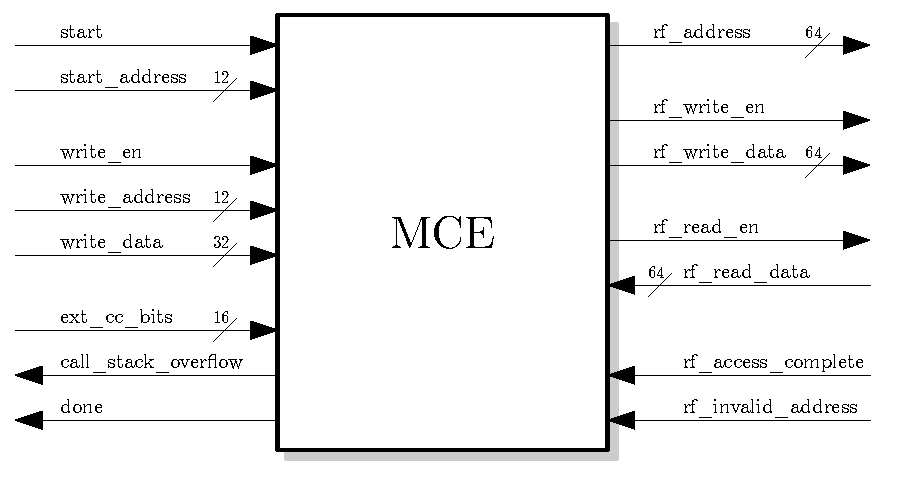
\includegraphics[width=1.0\textwidth,angle=0]{images/mce_black_box}
 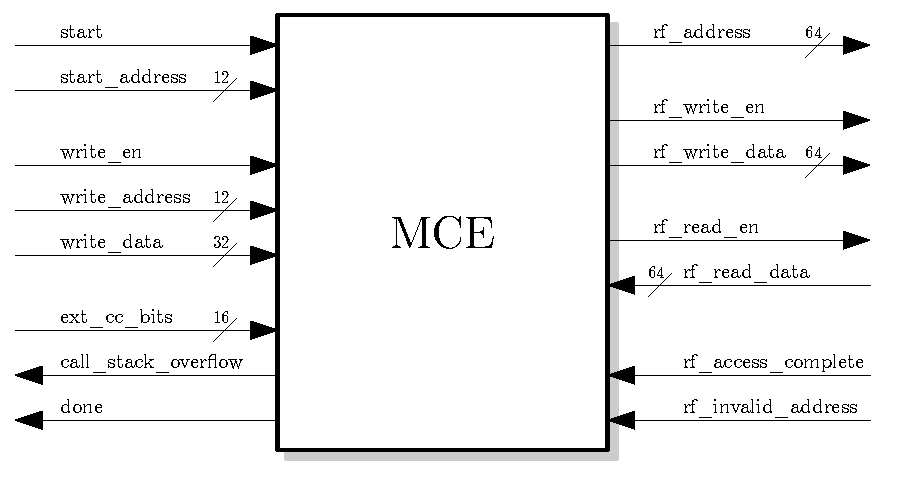
\includegraphics[scale=1.0]{images/mce_black_box}
 \caption{MCE Interface}
\label{fig:mce_inf}
\end{figure}

\subsubsection{Start Interface}

The start interface is used to begin the execution of a program in the MCE.
It consists of the \emph{start} and \emph{start\_address} signals.
When \emph{start} is asserted, the in  \emph{start\_address} specified address is loaded into the PC.
Additionally the MCE is started, if it is not already running.
Otherwise a jump to \emph{start\_address} is performed.

\subsubsection{Instruction Memory Interface}

Before a program can be started. The instructions have to be written into the instruction memory.
This is done via the instruction memory interface.
It consists of the \emph{write\_en}, \emph{write\_address} and \emph{write\_data} signals.
When \emph{write\_en} is asserted, the instruction specified in \emph{write\_data} is written into the instruction memory at the address given by \emph{write\_address}.

\subsubsection{External Condition Code Interface}

Via the external condition code interface, other components can apply condition code bits to the MCE by setting \emph{ext_cc_bits}.
These can then be used in the BCC instruction to decide, if a conditional branch shall be executed.

\subsubsection{Call Stack Overflow Interface}

The call stack has a limited size.
If the CALL instruction is executed, when the call stack is full, an overflow occurs and the MCE stops.
The call stack overflow interface is used to inform other modules about this by asserting \emph{call\_stack\_overflow}.
The signal stays asserted until the MCE is started again via the start interface.

\subsubsection{Done Interface}

When the STOP instruction is executed, the execution of the MCE is stopped.
To inform other modules about this, the done interface is used.
Additionally to stopping the MCE the \emph{done} signal is asserted.
It stays asserted until the MCE is started again via the start interface.

\subsubsection{Memory Interface}



\subsection{Hardware Architecture}



\begin{figure}[htb]
 \centering
 %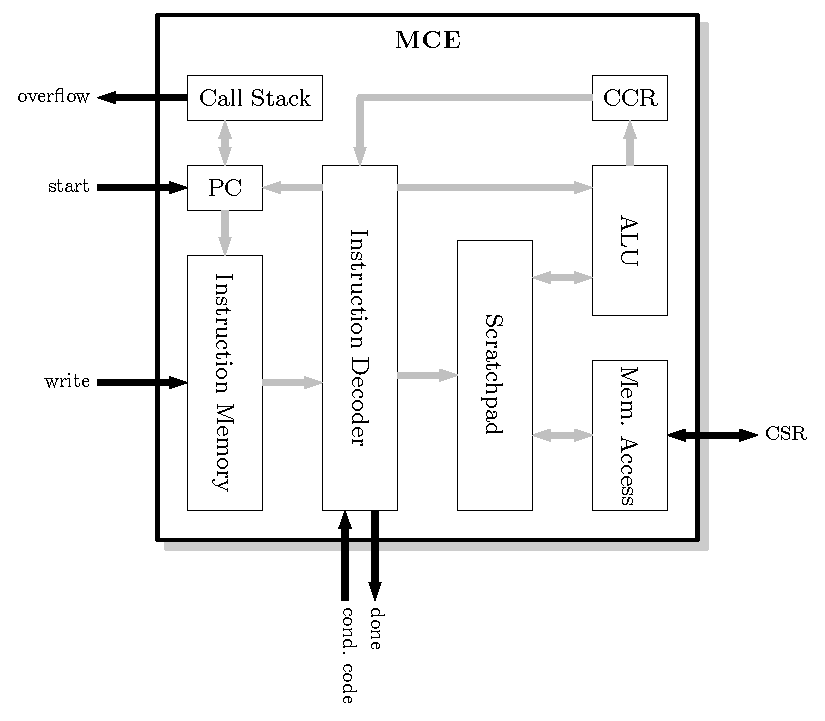
\includegraphics[width=1.0\textwidth,angle=0]{images/mce_block}
 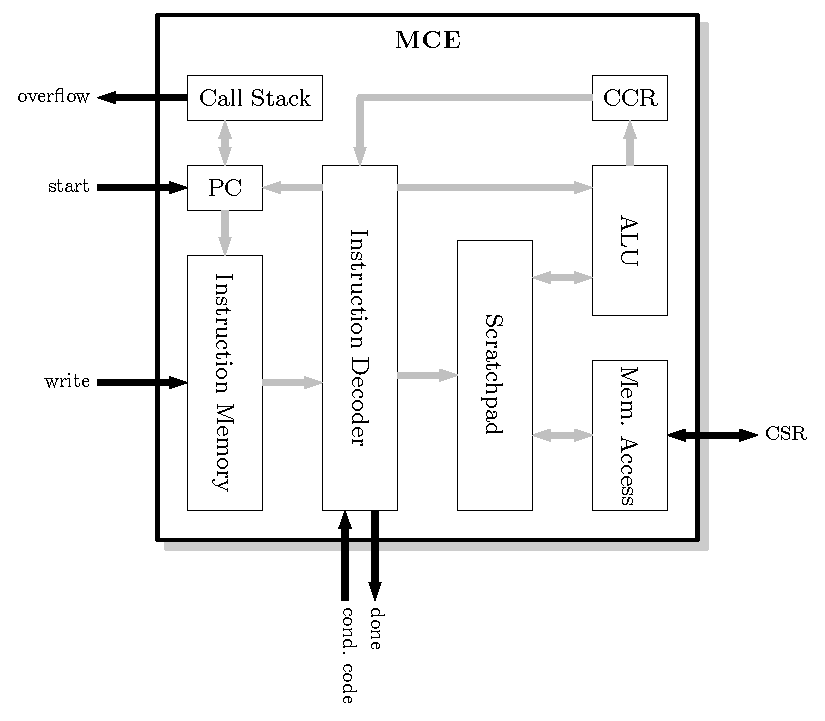
\includegraphics[scale=1.0]{images/mce_block}
 \caption{MCE Block Diagram}
\label{fig:mce_block}
\end{figure}

- 4 pipeline stages\\
- in-order\\
- interfaces\\
- image: black box / stages\\

\subsubsection{Instruction Memory}

- stores the instructions\\
- write interface\\
- 4kx32bit ram\\

\subsubsection{Program Counter}

- address pointer of the current instruction\\
- value is read each clock cycle\\
- updated to point to the next instruction\\
- control flow instruction can modify the pc\\
- execution starts at 'start' signal\\
- execution ends at STOP instruction

\subsubsection{Call Stack}

- stack that can hold up to 14 addresses\\
- CALL pushes address\\
- RET pops address\\
- overflow is passed to external interface\\
- overflow terminates program execution\\
- only stores pc, not scratchpad\\

\subsubsection{Scratchpad}

\begin{figure}[htb]
 \centering
 %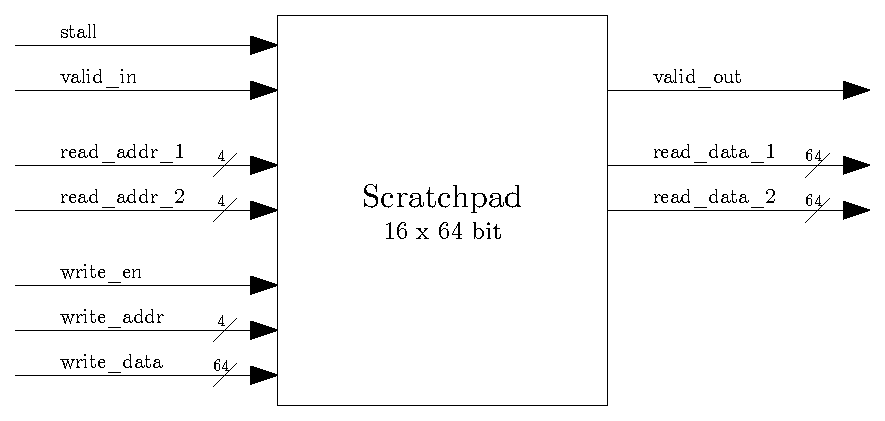
\includegraphics[width=1.0\textwidth,angle=0]{images/scratchpad_blackbox}
 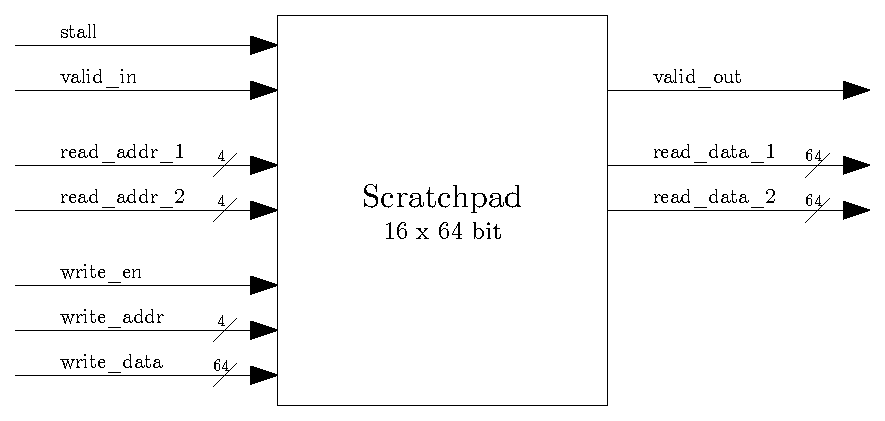
\includegraphics[scale=1.0]{images/scratchpad_blackbox}
 \caption{Scratchpad Interface}
\label{fig:scp_inf}
\end{figure}

- stores results of operations\\
- provides operands to operations\\
- data available next clk cycle\\
- 16x64bit register\\
- 4 bit address\\
- 1 write port (stage 3)\\
- written by ALU and memory interface\\
- 2 read ports (stage 1)\\
- data forwarding when same address is read/written\\


\subsubsection{Arithmetic Logic Unit}

- executes operations\\
- calculates results\\
- calculates condition code\\
- stage 2\\

\subsubsection{Memory Interface}

- access to the registerfile\\
- LDR read from memory\\
- STR write to memory\\
- stalls pipeline, when read/write conflict occurs\\
- stalls pipeline, when memory access, while pending access\\
- stage 2\\

\subsubsection{Condition Code Register}

\begin{figure}[htb]
 \centering
 %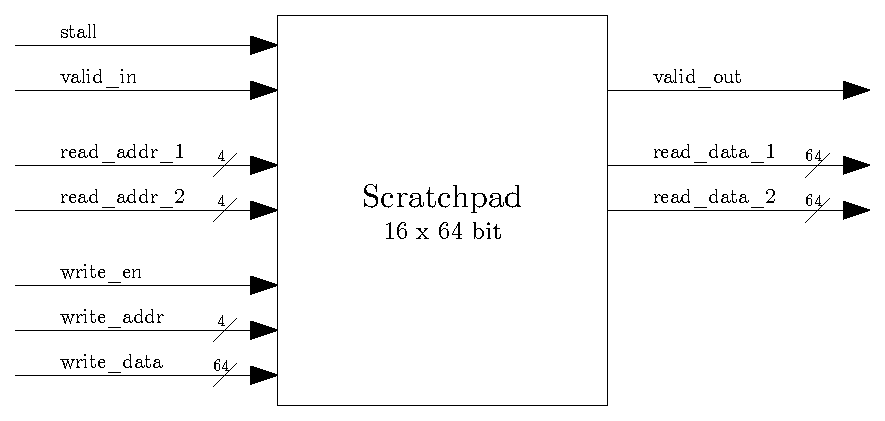
\includegraphics[width=1.0\textwidth,angle=0]{images/scratchpad_blackbox}
 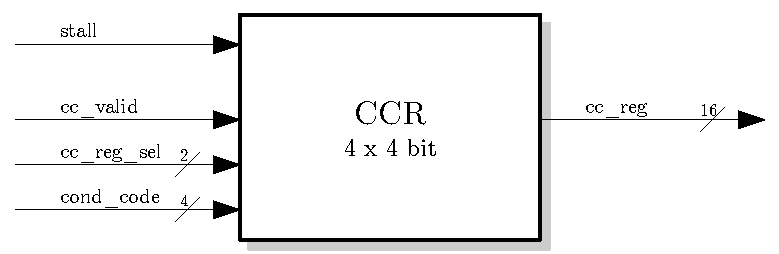
\includegraphics[scale=1.0]{images/ccr_blackbox}
 \caption{Condition Code Register Interface}
\label{fig:ccr_inf}
\end{figure}

- 4x4bit register\\
- stores condition code calculated by ALU\\
- only written by ALU\\
- each bit can be accessed directly to determine, if a GUARD instruction or BCC should be executed\\
- stage 3\\
- 3 instructions delay between writing and reading instruction\\




